\section{Spectrecoin Privacy Features}
Before we go on to explain some of the features and technologies of
Spectrecoin in more detail, we will give you a short overview of the
privacy technology used. The Spectrecoin blockchain is a ‘dual-coin’
system or a system where two distinct types of transaction outputs can
exist in the same block. Both non-private or standard UTXOs (hereafter
referred to as public coins or XSPEC) and private coins or ATXOs (hereafter
referred to as private coins or SPECTRE) exists side by side in the
block-chain. Transactions can be carried out with both public and private
coins and they are interchangeable and independent. We introduce the terms
XSPEC for the public coins spent in standard UTXO based transactions and
SPECTRE for the private coins spent in a confidential ATXO based
transactions using ring signatures. XSPEC is used in the PoSv3 consensus
mechanism and SPECTRE is used in the PoAS consensus mechanism.



\subsection{Dual Coin System}
The private coin ‘subsystem’ was inspired by the principles of the Zerocoin
protocol which can be summarised as ‘Anonymity by destruction / creation of
basecoins’, i.e. destroy / consume one base unit, create a private token
and create a proof that the user owns it and the system later agrees to
re-create one base coin from that proof when requested. The Zerocoin protocol
utilises a so called zero-knowledge proof (ZKP) to create the private coins
and to prove ownership. Zerocoin is computationally intense and requires a
trusted setup and we have recently seen that the Zerocoin protocol can be
subject to certain attacks due to what can be described as flaws in the
theory and 
implementation\footnote{https://www.chaac.tf.fau.eu/2018/04/12/zerocoinzcoinpivxzoinsmartcashhexxcoin-attack/}. 
Some well-known Zerocoin based cryptocurrencies
such as Zcoin, PIVX and NIX were forced to shut down their privacy system and
work to implement fixes.



The Spectrecoin network instead employs dual-key stealth address cryptography
to facilitate the creation of privacy maintaining \textbf{SPECTRE} coins on the
blockchain whilst consuming \textbf{XSPEC}. This is done without the trusted setup
required for Zerocoin and without using the computationally intense Zerocoin
cryptographic methods. Where the Zerocoin protocol use ZKP to anonymise and
unlink the transactions, 
\textbf{the Spectrecoin network use ring signatures}\footnote{https://people.csail.mit.edu/rivest/pubs/RST01.pdf/} 
\& \footnote{https://arxiv.org/pdf/1612.01188.pdf}.



\begin{figure}[h]
	\caption{Example of a parametric plot ($\sin (x), \cos(x), x$)}
	\centering
	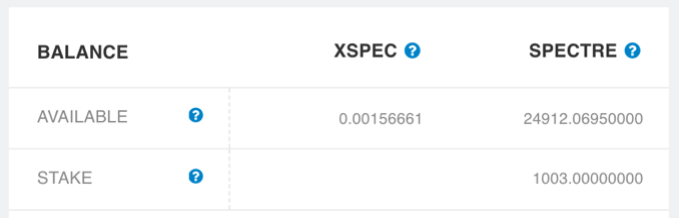
\includegraphics[width=0.5\textwidth]{Wallet-BalanceDualCoin.png}
\end{figure}



The ‘\textit{dual-coin}’ system can be seen as a feature allowing for complete
transparent transactions and network audit functions if needed but
without any privacy indebted overhead such as resource intensive
calculations. Privacy maintaining \textbf{SPECTRE} can ONLY be created by
consuming \textbf{XSPEC} at this time and the total supply on the network
will always be transparent. There is no ‘\textit{bleed through}’ between the
two types of transaction outputs and no compromise in privacy.



\subsection{XSPEC/SPECTRE Conversion}
Each user can convert (\textit{non-private}) \textbf{XSPEC} coins into (\textit{private}) coins, \textbf{SPECTRE}.
Users can then send \textbf{SPECTRE} to other users and split or merge the \textbf{SPECTRE} they
own \underline{in any way that preserves the total value}. Once \textbf{SPECTRE} has been created
and matured the user will also be able to stake in private through the PoAS
protocol. Users can also convert \textbf{SPECTRE} back into \textbf{XSPEC}, though in principle
this is not necessary: all transactions can be made in terms of \textbf{SPECTRE}.



\begin{figure}[h]
	\caption{Your wallet will show your \textbf{XSPEC} balance, your 
		\textbf{SPECTRE} balance and on top the total balance.}
	\centering
	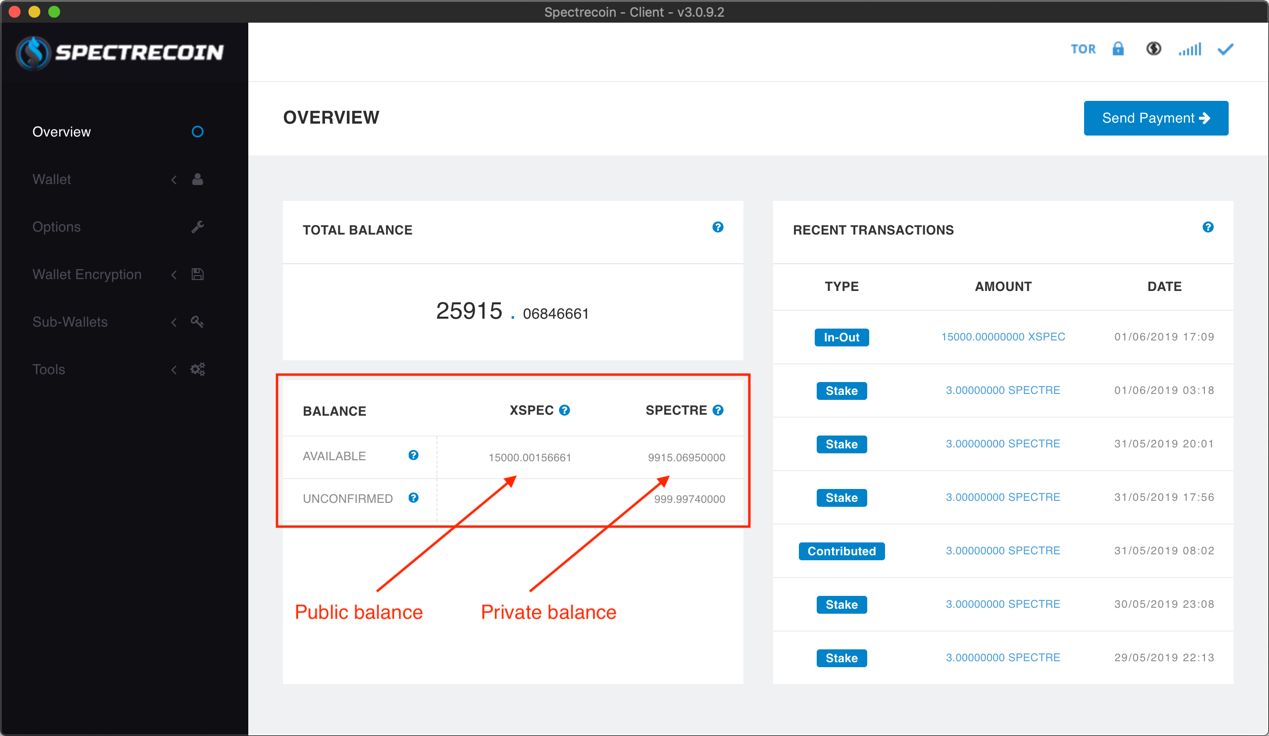
\includegraphics[width=\textwidth]{WalletUI-3x-2.png}
\end{figure}




The core privacy technology used in Spectrecoin is: 



\begin{description}
	\item[Recipient privacy:] Stealth addresses are used to protect the recipient’s privacy. (SPECTRE only)
	\item[Sender privacy:] Ring Signatures are used to protect the sender’s privacy. (SPECTRE only)
	\item[IP address privacy:] All Spectrecoin nodes run as TOR hidden services to protect users IP address.
	\item[Un-traceability:] for each incoming transaction all possible senders are equiprobable. (SPECTRE only)
	\item[Un-linkability:] for two outgoing transactions it is impossible to prove the same receiver. (SPECTRE only)
\end{description}
         



Now let’s have a look at the different features in some more detail in the
following sections. We aim to briefly explain the background and nature of
stealth addresses and ring-signatures and how this is used in Spectrecoin.
